To test if 
the LSTM layer could be replaced by 
another way of aggregating the convolutional layer outputs, three networks were constructed without any LSTM layer.

One of them, ``CM'' uses a stride of one and aggregates the results using a big max pooling layer.

Another one, ``CCM'' uses the same strategy, but includes another convolutional layer before the max pooling.

The last one, ``CD'', uses a bigger input window of 64 units, but with a smaller stride of 8 units. The output layer is a fully connected layer.

The results are shown in table \ref{tab:carvingnolstm}. The ``CL'' network is included for comparison.
These three networks produced similar results, but they are not as good as the ``CL'' network, as can be seen in figure
\ref{fig:nolstm}.


\begin{table*}[!ht]
    \centering
    \caption[No LSTM]{Comparison of models that do not use LSTM}
    \label{tab:carvingnolstm}
\begin{tabular}{r|r|r|r|r|r|r}
\hline
Name & Parameters & Blocks & Epochs & Time & Training          & Validation          \\       
     &            &        &        &         &          accuracy &            accuracy \\ \hline\hline

CL      & 24663     & all   & 159   & 10m00s    & 0.83  & 0.789 \\\hline
CM      & 24579     & all   & 98    & 10m01s    & 0.806 & 0.796 \\\hline
CCM     & 24600     & all   & 93    & 10m04s    & 0.778 & 0.786 \\\hline
CD      & 1059587   & all   & 144   & 10m00s    & 0.758 & 0.751 \\\hline
\end{tabular}
\end{table*}

\begin{figure}[htb!]
\centering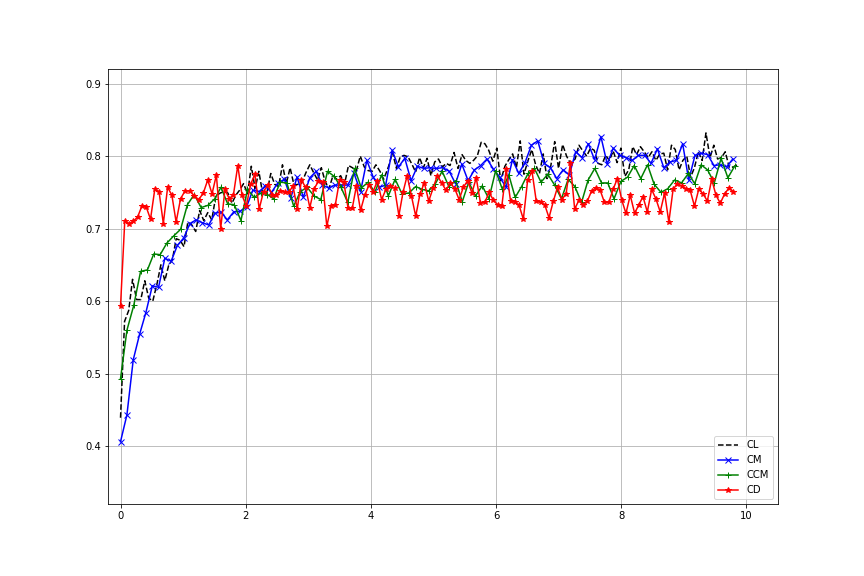
\includegraphics[width=0.50\textwidth]{content/CL-CM-CCM-CD.png}
\caption[No LSTM]{\label{fig:nolstm}Comparison of models that do not use LSTM - validation accuracy vs. time(minutes)}%
\end{figure}

